%%%%%%%%%%%%%%%%%%%%%%%%%%%%%%%%%%%%%%%%%%%
%%%%%%%%%%%%%%%%%%%%%%%%%%%%%%%%%%%%%%%%%%%
%%%%%%%%%%%%%%% CHAPTER 07 %%%%%%%%%%%%%%%%


\section{Modelagem: sistemas elétricos}

\frame{
\frametitle{Variáveis}
\begin{block}{Símbolos utilizados}
\begin{itemize}
    \item Os símbolos para as variáveis básicas utilizadas para descrever o comportamento de um sistema elétrico são:
    \begin{itemize}
        \item $e$, \textbf{tensão} em volts (V)
        \item $i$, \textbf{corrente} em amperes (A)
        \item $q$, \textbf{carga elétrica} em coulombs (C)
        \item $\phi$, \textbf{fluxo magnético} em weber (W)
    \end{itemize}
\end{itemize}
\end{block}
}

\frame{
\frametitle{Variáveis}
\begin{block}{Relação entre as variáveis}
\begin{itemize}
    \item A corrente pode ser encontrada derivando (no tempo) a carga elétrica, isto é,
$$i = \dfrac{dq}{dt}$$
e
$$q(t) = q(t_0) + \int_{t_0}^{t} i(\lambda) d\lambda$$
    \item A representação da corrente é feita com a seta apontando para direção onde a \textbf{carga positiva} (íons positivos) flui.
\end{itemize}
\end{block}
}

\frame{
\frametitle{Leis dos elementos}
\begin{block}{Resistor}
\begin{itemize}
    \item O resistor é um elemento \textbf{passivo} que dissipa energia do circuito. Um resistor linear é aquele onde a relação entre corrente e tensão é diretamente proporcional, obedecendo a \textbf{lei de Ohm}:
    $$e = Ri$$
    \item A resistência de um corpo de comprimento $l$ e área de secção transversal $A$ feito de um material com resistividade $\rho$ é:
    $$R = \dfrac{\rho l}{A}$$
    \item A potência ($\bm{p}$) dissipada em forma de calor pode ser expressa como
    $$p = Ri^2$$
\end{itemize}
\end{block}
}

\frame{
\frametitle{Leis dos elementos}
\begin{block}{Capacitor}
\begin{itemize}
    \item O capacitor é um elemento \textbf{passivo} que armazena energia em forma de campo elétrico. Um capacitor linear possui a seguinte relação:
    $$q = Ce$$
    \item Diferenciando a equação acima e lembrando que $\dot{q} = i$, vem:
    $$i = C\dfrac{de}{dt}$$
    \item Integrando e expressando a tensão nos terminais do capacitor em termo da corrente, temos:
    $$e(t) = e(t_0) + \dfrac{1}{C}\int_{t_0}^{t} i(\lambda) d\lambda$$
\end{itemize}
\end{block}
}

\frame{
\frametitle{Leis dos elementos}
\begin{block}{Indutor}
\begin{itemize}
    \item O indutor é um elemento \textbf{passivo} que armazena energia em forma de campo magnético. Um indutor linear possui a seguinte relação:
    $$e = L \dfrac{di}{dt}$$
    \item Integrando a equação acima, vem:
     $$i(t) = i(t_0) + \dfrac{1}{L}\int_{t_0}^{t} e(\lambda) d\lambda$$
\end{itemize}
\end{block}
}

\frame{
\frametitle{Leis dos elementos}
\centerline{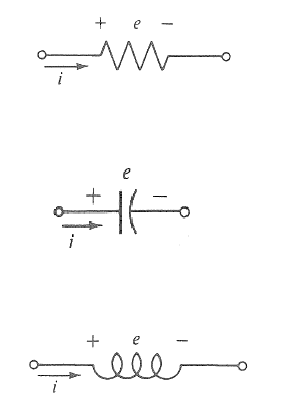
\includegraphics[width=0.4\linewidth]{Figuras/Ch07/fig1.PNG}}
}

\frame{
\frametitle{Leis dos elementos}
\begin{block}{Fonte}
\begin{itemize}
    \item As fontes de corrente e tensão ideias são elementos \textbf{ativos} de um circuito elétrico, pois elas fornecem energia ao mesmo.
    \item Uma fonte de tensão ideal fornece determinada tensão \textbf{independente} da corrente que pode fluir no circuito. O mesmo acontece com uma fonte de corrente ideal, que fornece uma determinada corrente independente da tensão que possa ser necessária.
\end{itemize}
\end{block}
\centerline{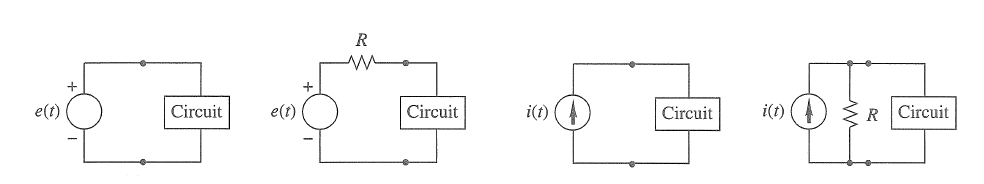
\includegraphics[width=1.2\linewidth]{Figuras/Ch07/fig2.PNG}}
}

\frame{
\frametitle{Interconectando as leis}
\begin{block}{LKT}
\begin{itemize}
    \item A \textbf{lei de Kirchhoff para tensão} (LKT) nos diz que em um \textit{loop} a soma algébrica de todas as tensões nos elementos deve ser igual a zero.
$$\boxed{\sum_{j}^{} e_j = 0}$$
\end{itemize}
\end{block}
}

\frame{
\frametitle{Interconectando as leis}
\begin{block}{LKT - Exemplo}
\begin{itemize}
    \item Considerando o sentido \textbf{anti-horário}, e partindo do nó $A$ temos:
    $$e_1 + e_2 - e_3 - e_4 = 0$$
    \item Considerando o sentido \textbf{horário}, e partindo do nó $A$ temos:
    $$e_4 + e_3 - e_2 - e_1 = 0$$
\end{itemize}
\end{block}
\centerline{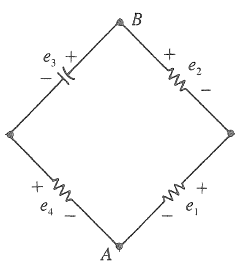
\includegraphics[width=0.32\linewidth]{Figuras/Ch07/fig3.PNG}}
}

\frame{
\frametitle{Interconectando as leis}
\begin{block}{LKC}
\begin{itemize}
    \item A \textbf{lei de Kirchhoff para corrente} (LKC) nos diz que em um \textit{nó} a soma algébrica de todas as correntes deve ser igual a zero.
$$\boxed{\sum_{j}^{} i_j = 0}$$
\end{itemize}
\end{block}
}

\frame{
\frametitle{Interconectando as leis}
\begin{block}{LKC - Exemplo}
\begin{itemize}
    \item Considerando que a corrente que sai de um nó é \textbf{positiva}, e a que entra em um nó é \textbf{negativa}, temos:
    $$\dfrac{1}{R}(e_A - e_B) + i_2(0) + \dfrac{1}{L}\int_{0}^{t} (e_A - e_D) d\lambda + C(\dot{e}_A - \dot{e}_F) = 0$$
\end{itemize}
\end{block}
\centerline{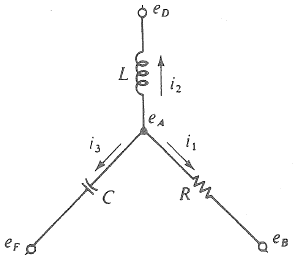
\includegraphics[width=0.35\linewidth]{Figuras/Ch07/fig4.PNG}}
}

\frame{
\frametitle{Exemplo $\#01$ - circuito RLC série}
\centerline{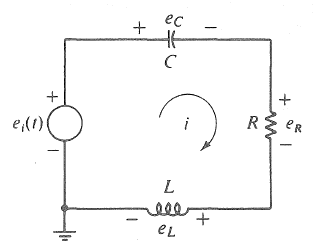
\includegraphics[width=0.4\linewidth]{Figuras/Ch07/fig5.PNG}}
\begin{block}{Problema}
\begin{itemize}
    \item Por uma simples análise da LKC percebemos que a corrente $i$ é a mesma em todos os elementos do circuito, logo eles estão conectados em \textbf{série}.
    \item Aplicando agora a LKT, obtemos:
    $$-e_R - e_L + e_i(t) - e_C = 0 \implies e_R + e_L + e_C = e_i(t)$$
\end{itemize}
\end{block}
}

\frame{
\frametitle{Exemplo $\#01$ - circuito RLC série}
\begin{block}{EDO}
\begin{itemize}
    \item Substituindo a lei individual de cada elemento na última equação, temos:
    $$Ri + L\dfrac{di}{dt} + e_C(0) + \dfrac{1}{C}\int_{0}^{t} i(\lambda) d\lambda = e_i(t)$$
    \item Derivando e rearrumando os termos, chega-se em:
    $$L\dfrac{d^2i}{dt^2} + R\dfrac{di}{dt} + \dfrac{1}{C}i = \dot{e}_i$$
\end{itemize}
\end{block}
}

\frame{
\frametitle{Exemplo $\#02$ - circuito RLC paralelo}
\centerline{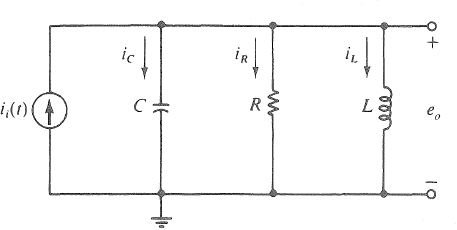
\includegraphics[width=0.5\linewidth]{Figuras/Ch07/fig6.PNG}}
\begin{block}{Problema}
\begin{itemize}
    \item Por uma simples análise da LKT percebemos que a tensão $e_0$ é a mesma em todos os elementos do circuito, logo eles estão conectados em \textbf{paralelo}.
    \item Aplicando agora a LKC, obtemos:
    $$i_1(t) - i_C - i_R - i_L = 0 \implies i_R + i_L + i_C = i_i(t)$$
\end{itemize}
\end{block}
}

\frame{
\frametitle{Exemplo $\#02$ - circuito RLC paralelo}
\begin{block}{EDO}
\begin{itemize}
    \item Substituindo a lei individual de cada elemento na última equação, temos:
    $$\dfrac{1}{R}e_0 + i_L(0) + \dfrac{1}{L}\int_{0}^{t} e_0(\lambda) d\lambda + C\dot{e}_0 = i_i(t)$$
    \item Derivando e rearrumando os termos, chega-se em:
    $$C\ddot{e}_0 + \dfrac{1}{R}\dot{e_0} + \dfrac{1}{L}e_0 = \dfrac{di_i}{dt}$$
\end{itemize}
\end{block}
}

\frame{
\frametitle{Exemplo $\#03$ - circuito com múltiplas malhas}
\centerline{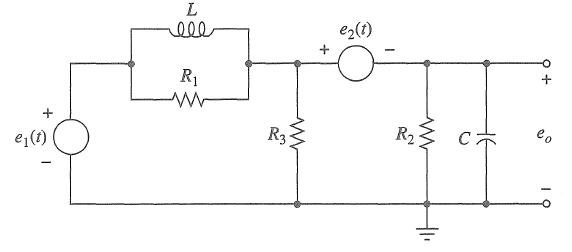
\includegraphics[width=0.55\linewidth]{Figuras/Ch07/fig7.PNG}}
\begin{block}{Problema}
\begin{itemize}
    \item Para a análise deste circuito, devemos notar a presença de \textbf{dois nós}:
    \begin{itemize}
        \item $\bm{e_0}$ do lado direito na junção entre $C$ e $R_2$.
        \item $\bm{e_0+e_2(t)}$ entre $e_2(t)$ e $R_3$ (aplicando LKT).
    \end{itemize}
    \item Considerando que no nó $\bm{e_0}$ saem as correntes $i_{R_2}$, $i_C$ e $i_2$ (a que passa pela fonte $e_2(t)$), temos, ao aplicar a LKC, o seguinte:
    $-i_C - i_{R_2} - i_2 = 0 \implies i_C + i_{R_2} + i_2 = 0$
    \item Considerando que no nó $\bm{e_0+e_2(t)}$ saem as correntes $i_{R_1}$, $i_{R_3}$ e $i_L$, e chega a corrente $i_2$, temos, ao aplicar a LKC, o seguinte:
    $i_2 -i_{R_3} - i_{R_1} - i_L = 0 \implies i_2 = i_{R_3} + i_{R_1} + i_L$
\end{itemize}
\end{block}
}

\frame{
\frametitle{Exemplo $\#03$ - circuito com múltiplas malhas}
\begin{block}{Análise}
\begin{itemize}
    \item Substituindo a segunda equação na primeira, chegamos a:
    $$i_C + i_{R_2} + i_{R_3} + i_{R_1} + i_L = 0$$
    \item As leis para cada elemento acima podem ser escritas como sendo:
    $$i_{R_1} = \dfrac{1}{R_1}[e_0 + e_2(t) - e_1(t)]$$
    $$i_{R_2} = \dfrac{1}{R_2}e_0$$
    $$i_{R_3} = \dfrac{1}{R_3}[e_0 + e_2(t)]$$
    $$i_C = C\dot{e}_0$$
    $$i_L = i_L(0) + \dfrac{1}{L}\int_{0}^{t} (e_0 + e_2 - e_1) d\lambda$$
\end{itemize}
\end{block}
}

\frame{
\frametitle{Exemplo $\#03$ - circuito com múltiplas malhas}
\begin{block}{EDO}
\begin{itemize}
    \item Substituindo todas as relações na equação obtida, derivando-a e simplificando-a, temos a seguinte EDO:
    $$C\ddot{e}_0 + \Big(\dfrac{1}{R_1} + \dfrac{1}{R_2} + \dfrac{1}{R_3}\Big)\dot{e}_0 + \dfrac{1}{L}e_0 = \dfrac{1}{R_1}\dot{e}_1 - \Big(\dfrac{1}{R_1} + \dfrac{1}{R_3}\Big)\dot{e}_2 + \dfrac{1}{L}[e_i(t) - e_2(t)]$$
    \item Esta EDO de \textbf{segunda ordem} relaciona a saída $e_0$ com as duas entradas $e_1(t)$ e $e_2(t)$.
    \item Geralmente, a ordem da EDO é igual ao número de \textbf{elementos armazenadores de energia}, que neste caso são \textbf{dois}: um capacitor e um indutor.
\end{itemize}
\end{block}
}

\frame{
\frametitle{Exemplo $\#04$ - circuito resistivo}
\centerline{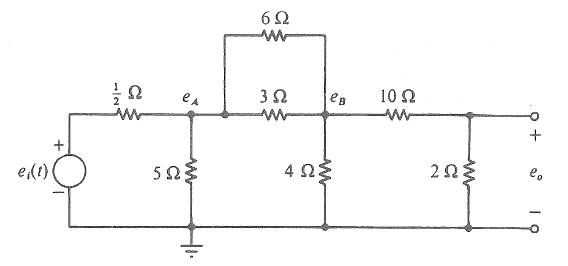
\includegraphics[width=0.7\linewidth]{Figuras/Ch07/fig8.PNG}}
\begin{block}{Problema}
\begin{itemize}
    \item Para determinar o valor de $\bm{e_0}$ no circuito, deve-se associar as resistências em série e em paralelo, e depois relacionar $\bm{e_0}$ com $\bm{e_A}$ e $\bm{e_B}$ por meio da regra de divisor de tensão.
\end{itemize}
\end{block}
}

\frame{
\frametitle{Exemplo $\#04$ - circuito resistivo}
\centerline{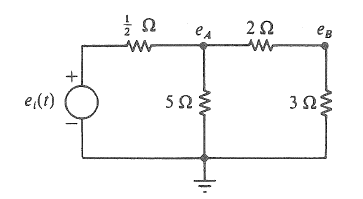
\includegraphics[width=0.6\linewidth]{Figuras/Ch07/fig9.PNG}}
\begin{block}{Análise}
\begin{itemize}
    \item Após algumas reduções série-paralelo, o circuito acima é obtido.
    \begin{itemize}
        \item $\SI{6}{\ohm} \parallel \SI{3}{\ohm} = \SI{2}{\ohm}$
        \item $\SI{10}{\ohm} + \SI{2}{\ohm} = \SI{12}{\ohm}$
        \item $\SI{12}{\ohm} \parallel \SI{4}{\ohm} = \SI{3}{\ohm}$
    \end{itemize}
\end{itemize}
\end{block}
}

\frame{
\frametitle{Exemplo $\#04$ - circuito resistivo}
\centerline{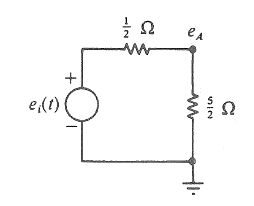
\includegraphics[width=0.4\linewidth]{Figuras/Ch07/fig10.PNG}}
\begin{block}{Análise}
\begin{itemize}
    \item O próximo passo é reduzir ainda mais a associação e determinar $\bm{e_A}$ por meio da regra de divisor de tensão:
    $$e_A = \dfrac{5/2}{1/2 + 5/2}e_i(t) = \dfrac{5}{6}e_i(t)$$
\end{itemize}
\end{block}
}

\frame{
\frametitle{Exemplo $\#04$ - circuito resistivo}
\centerline{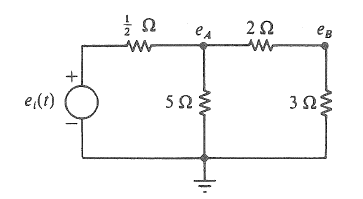
\includegraphics[width=0.6\linewidth]{Figuras/Ch07/fig9.PNG}}
\begin{block}{Análise}
\begin{itemize}
    \item De possa dessa informação, temos que:
    $$e_B = \dfrac{3}{3 + 2}e_A(t) = \dfrac{1}{2}e_i(t)$$
\end{itemize}
\end{block}
}

\frame{
\frametitle{Exemplo $\#04$ - circuito resistivo}
\centerline{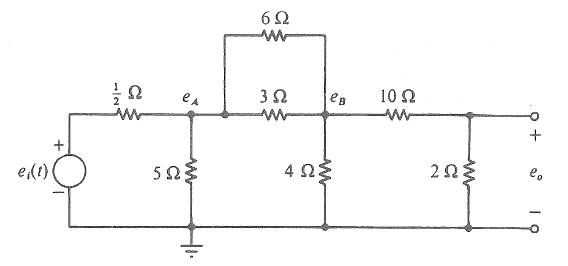
\includegraphics[width=0.7\linewidth]{Figuras/Ch07/fig8.PNG}}
\begin{block}{Análise}
\begin{itemize}
    \item Então, utilizando o diagrama original do circuito, chegamos a:
    $$e_0 = \dfrac{2}{2+10}e_B = \dfrac{1}{12}e_i(t)$$
\end{itemize}
\end{block}
}

\frame{
\frametitle{Exemplo $\#05$ - AmpOp inversor}
\begin{block}{Fundamentação teórica}
\begin{itemize}
    \item Um \textbf{amplificador operacional} (AmpOp) é um circuito eletrônico que possui duas entradas independentes e uma saída.
    \item A entrada marcada com um sinal de menos é chamada de \textbf{entrada inversora}, e a marcada com um sinal de mais é chamada de \textbf{entrada não inversora}
    \item O resistor de entrada ($\bm{r_n}$) possui valores típicos na faixa de milhões de ohms, enquanto o resistor de saída ($\bm{r_0}$) não passa da casa das dezenas.
\end{itemize}
\end{block}
\centerline{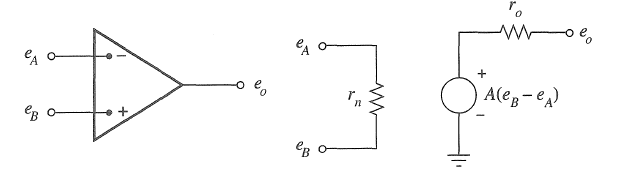
\includegraphics[width=0.8\linewidth]{Figuras/Ch07/fig11.PNG}}
}

\frame{
\frametitle{Exemplo $\#05$ - AmpOp inversor}
\begin{block}{Fundamentação teórica}
\begin{itemize}
    \item Tais considerações permitem redesenhar o modelo do AmpOp como o descrito abaixo, assumindo que \textbf{nenhuma corrente pode fluir no dispositivo pela esquerda}.
    \item A constante de amplificação do AmpOp, $\bm{A}$, é extremamente grande.
    $$e_0 = A(e_B - e_A)$$
    \item Como $e_0$ deve ser finito, temos que a diferença de tensão entre os terminais de entrada do AmpOp tende a zero, i.e., $e_A = e_B$. Este conceito é chamado de \textbf{curto virtual}.
\end{itemize}
\end{block}
\centerline{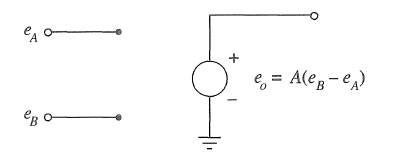
\includegraphics[width=0.6\linewidth]{Figuras/Ch07/fig12.PNG}}
}

\frame{
\frametitle{Exemplo $\#05$ - AmpOp inversor}
\centerline{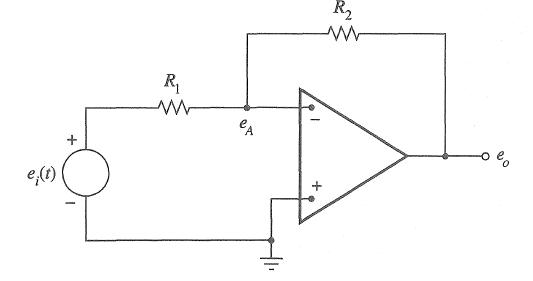
\includegraphics[width=0.6\linewidth]{Figuras/Ch07/fig13.PNG}}
\begin{block}{Problema}
\begin{itemize}
    \item Analisando o circuito temos que $e_B = 0$ e usando o conceito de curto virtual nos leva a $e_A = 0$.
    \item Aplicando a LKC no nó $\bm{e_A}$:
    $$-\dfrac{1}{R_1}(e_1 - e_A) + \dfrac{1}{R_2}(e_A - e_0) = 0$$
\end{itemize}
\end{block}
}

\frame{
\frametitle{Exemplo $\#05$ - AmpOp inversor}
\begin{block}{Problema}
\begin{itemize}
    \item Substituindo $e_A = 0$ e rearranjando os termos, vem:
    $$\dfrac{1}{R_1}e_1 = \dfrac{1}{R_2}(- e_0)$$
    $$e_0 = - \dfrac{R_2}{R_1}e_1$$
\end{itemize}
\end{block}
}

\frame{
\frametitle{Exemplo $\#06$ - AmpOp não inversor}
\centerline{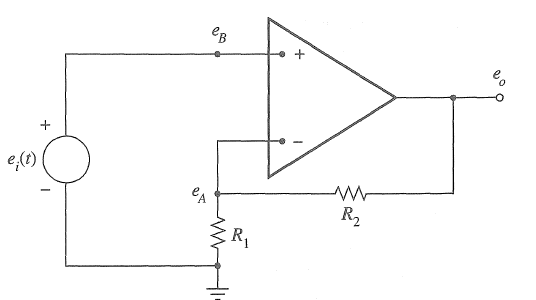
\includegraphics[width=0.6\linewidth]{Figuras/Ch07/fig14.PNG}}
\begin{block}{Problema}
\begin{itemize}
    \item Analisando o circuito temos que $e_B = e_i(t)$ e usando o conceito de curto virtual nos leva a $e_A = e_i(t)$.
    \item Aplicando a LKC no nó $\bm{e_A}$:
    $$\dfrac{1}{R_1}(e_A - 0) + \dfrac{1}{R_2}(e_A - e_0) = 0$$
\end{itemize}
\end{block}
}

\frame{
\frametitle{Exemplo $\#06$ - AmpOp não inversor}
\begin{block}{Problema}
\begin{itemize}
    \item Substituindo $e_A = e_i$ e rearranjando os termos, vem:
    $$\dfrac{1}{R_1}e_i = -\dfrac{1}{R_2}(e_i - e_0)$$
    $$e_0 = \Big(1 + \dfrac{R_2}{R_1}\Big)e_1$$
\end{itemize}
\end{block}
}

\frame{
\frametitle{Exercícios}
\begin{block}{}
01. Para o sistema mostrado abaixo (à esquerda), encontre a EDO que relaciona a saída $e_0$ com a entrada $i_i(t)$.

\vspace{0.5cm}

02. Repita para o sistema mostrado à direita, encontre a EDO que relaciona a saída $e_0$ com a entrada $e_i(t)$.
\end{block}
\centerline{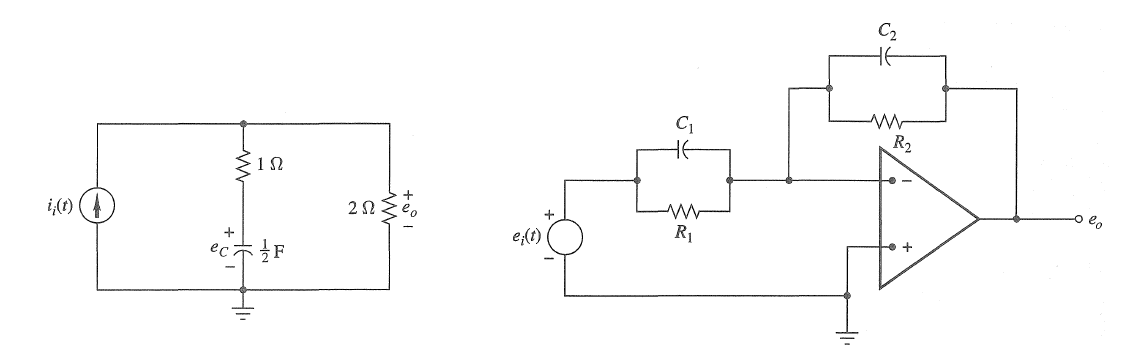
\includegraphics[width=1.2\linewidth]{Figuras/Ch07/fig15.PNG}}
}


\frame{
\frametitle{Referências e exercícios complementares}
\begin{itemize}
\item CLOSE, Charles M.; FREDERICK, Dean K.; NEWELL, Jonathan C. Modeling and Analysis of Dynamic Systems, 3 ed. John Wiley \& Sons, 2003.
\end{itemize}
\centering{\alert{Página 177 - \textbf{Capítulo 6}}} \\
}